%use in documents with \subfile{tex/intro}
\documentclass[../../master.tex]{subfiles}

\begin{document}

\subsubsection{Sequence Designs}
\label{ssub:results:designs}

For each set of sequence constraints (see \autoref{tab:constraintsets}), $n = 1000$ RNA sequence were designed using the pipeline described in \autoref{sub:methods:design_pipeline}.



\paragraph{Designs with constrained Structure Prediction and Objective Function.}
\label{par:results:constrained_ned}

The initially designed sequences of the constraint set \texttt{proto} followed the same design approach as the designs examined in this section.
However, since the former differed in the reference sequence and target structure from the other constraint sets, they were considered separately in \autoref{sub:appendix:protodesigns}.

To get an overview of the nucleotide composition of all the designed sequences of a particular constraint set, sequence logo plots were generated (Figure \ref{fig:logos}), displaying the information content per position \parencite{schneider_information_1986}. 
Here, no prior underlying nucleotide distribution was assumed.
Expectedly, positions with fixed nucleotides dominate the appearance in these plots.

Positions unconstrained in both \texttt{minimal} and \texttt{complete} tended to be of quite diverse composition, with only a few isolated positions having a single dominating nucleotide identity. 
Overall, \autoref{fig:logos:a} and \ref{fig:logos:b} display largely similar nucleotide compositions where no nucleotide identities were enforced by sequence constraints.
Positions that were constrained in \texttt{complete} but not in \texttt{minimal}, show no obvious overlap in their nucleotide composition in Figure \ref{fig:logos}, reassuring the orthogonality of tertiary interactions and secondary structure.

These observations indicate that a diverse range of possible sequences was generated in the design process. 
The inclusion of sequence constraints to account for tertiary interactions did not create biases interfering with the design process, apart from the fixed positions.

\begin{figure}[!ht]
	\centering
	\begin{subfigure}[t]{0.8\textwidth}
		\centering
		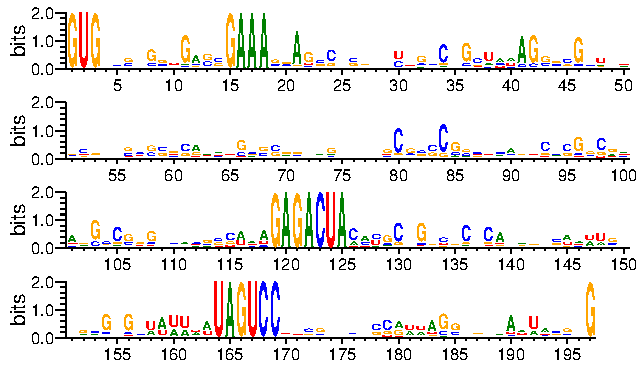
\includegraphics[trim=0 0 0 0, clip, width=\textwidth]{pic/results/designs/logos/logo-minimal.pdf}
		\caption{\texttt{minimal} constraint set.
		}\label{fig:logos:a}
	\end{subfigure}%
	\\
	\begin{subfigure}[t]{0.8\textwidth}
		\centering
		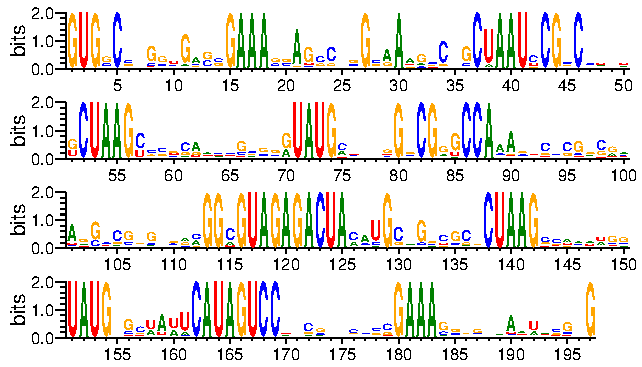
\includegraphics[trim=0 0 0 0, clip, width=\textwidth]{pic/results/designs/logos/logo-complete.pdf}
		\caption{\texttt{complete} constraint set.
		}\label{fig:logos:b}
	\end{subfigure}
	\caption[Nucleotide Composition of Designs (Constrained Approach)]{
		Sequence logos of 
		\begin{enumerate*}[label={(\alph*)}, font={\bfseries}]
			\item sequences designed with the \texttt{minimal} constraint set ($n = 1000$)
			\item sequences designed with the \texttt{complete} constraint set ($n = 1000$).
		\end{enumerate*}
		Nucleotides were colored according to their identity.
		Positions with an information content of \unit[2]{bit} correspond to the sequence constraints.
	}\label{fig:logos}
\end{figure}

Indeed, the sequence constraints applied in the design process seem to be the primary cause for reduced diversity:
The Hamming distance, i.e. the number of point mutations, relative to the native sequence is shown in \autoref{fig:stats_constrained:a} for both sets of sequence designs.

Considering the total number of fixed positions for each constraint set (see \autoref{tab:constraintsets}) and assuming to correctly guess \unit[25]{\%} of nucleotide positions of the native reference sequence by choosing from equiprobable nucleotides, an average Hamming distance of $\nicefrac{3}{4} (197 - 67) = 97.5$ for the \texttt{complete} set and $\nicefrac{3}{4} (197 - 21) = 132$ for the \texttt{minimal} set respectively, could be expected.

Despite being a very rough simplification, this is surprisingly close to, albeit still overestimating, the median values of \autoref{fig:stats_constrained:a}. 

Since the minimization of the normalized ensemble defect was stopped at $0.05$, the outcome of \autoref{fig:stats_constrained:b} was expected.
However, outliers arise due to the application of additional stop conditions (see \autoref{par:methods:pipelineoverview}).

As seen in \autoref{fig:stats_constrained:c}, the predicted minimum free energy structures were generally closer to the target structure than the same predictions for the native sequence (cf. \autoref{tab:predictionstats}).
Here, the constrained \texttt{RNAfold} performed the best, which seems plausible given that its predictions were used in the design process itself.
Nevertheless, the median base pair distance of predictions made by \texttt{pKiss} with modified pseudoknot penalty was still small and therefore seen as practical validation of the design approach.
Structure predictions using \texttt{RNAPKplex} were in the same range as \texttt{pKiss}, although showing a higher median value.

\begin{figure}[!ht]
	\centering
	\begin{subfigure}[t]{0.2\textwidth}
		\centering
		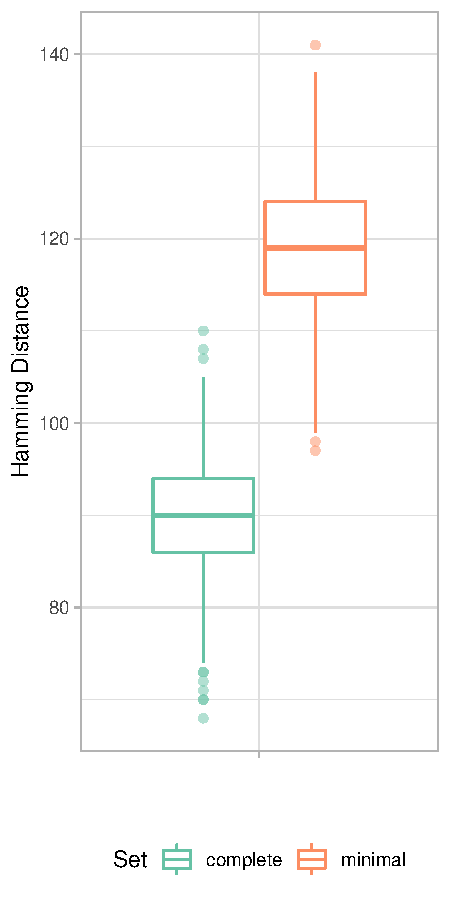
\includegraphics[width=\textwidth]{pic/results/designs/boxplots/const-hamming-boxplot.pdf}
		\caption{Hamming distance to the native sequence as a measure of sequence similarity.
		}\label{fig:stats_constrained:a}
	\end{subfigure}%
	\begin{subfigure}[t]{0.2\textwidth}
		\centering
		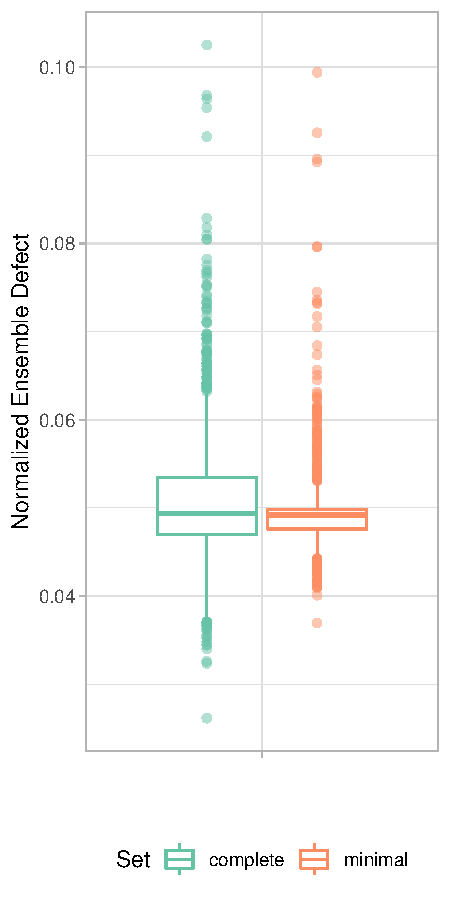
\includegraphics[width=\textwidth]{pic/results/designs/boxplots/const-score-boxplot.pdf}
		\caption{the normalized ensemble defect to the pseudoknot-free target structure.
		}\label{fig:stats_constrained:b}
	\end{subfigure}%
	\begin{subfigure}[t]{0.27\textwidth}
		\centering
		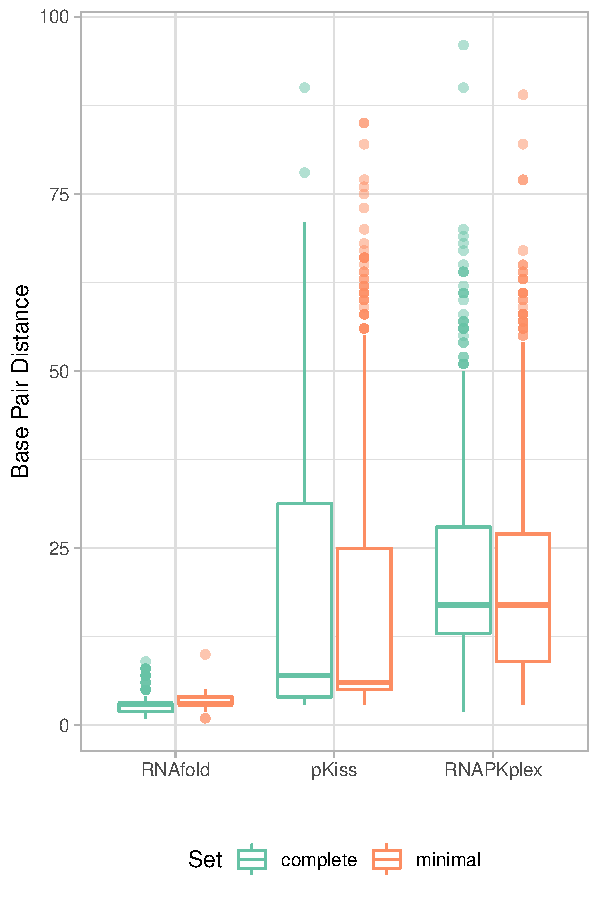
\includegraphics[width=\textwidth]{pic/results/designs/boxplots/const-bp-boxplot.pdf}
		\caption{Base pair distances relative to the target structure. For predictions made by \texttt{RNAfold}, base pairs of P7 were assumed to be present.
		}\label{fig:stats_constrained:c}
	\end{subfigure}
	\begin{subfigure}[t]{0.27\textwidth}
		\centering
		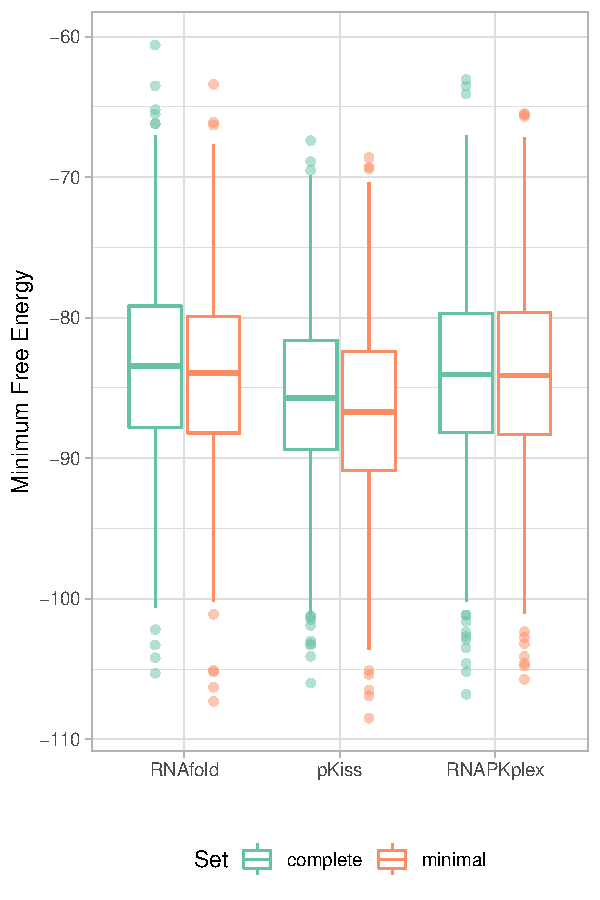
\includegraphics[width=\textwidth]{pic/results/designs/boxplots/const-mfe-boxplot.pdf}
		\caption{Free Energy of the predicted structures.  \texttt{RNAfold} values were corrected by the energy of the assumed base pairs in P7 (\autoref{fig:p7energy:a}).
		}\label{fig:stats_constrained:d}
	\end{subfigure}
	\caption[Properties of Sequence Designs (Constrained Approach)]{
		Metrics computed for $n = 1000$ sequences designed using the constraint sets \texttt{minimal} and \texttt{complete} respectively. Note that computations done by \texttt{RNAfold} or \texttt{ViennaRNA} were subject to structural constraints as described in \autoref{ssub:methods:rnafold}.
	}\label{fig:stats_constrained}
\end{figure}

Interestingly, in \autoref{fig:stats_constrained:c}, the difference between the \texttt{complete} and \texttt{minimal} set seemed relatively small, which may indicate that, even in the \texttt{complete} set, the total number of constraints was still small enough to explore the sequence space somewhat sufficiently.

Moreover, the free energies of the predicted structures as depicted in \autoref{fig:stats_constrained:d} were relatively consistent across the three different tools, as well as between both constraint sets.
On its own, this seemed surprising, considering that different pseudoknot penalties were applied.
Then again, it is consistent with the observation of similarly predicted free energy for the native \textit{Azoarcus} sequence itself as already established in \autoref{ssub:results:azopred} (cf. \autoref{tab:predictionstats}).

As written in \autoref{ssub:methods:selection}, the designed sequences were considered robust if the three MFE predictions were similar in the sense that their average base pair distance to the target was small.

This way, one of the best and one of the worst sequence designs were selected, and their base pair probability matrices were computed using the McCaskill algorithm implemented in \texttt{ViennaRNA} (Figure \ref{fig:bpp_pseven}).

\begin{figure}[!ht]
	\centering
	\begin{subfigure}[t]{0.5\textwidth}
		\centering
		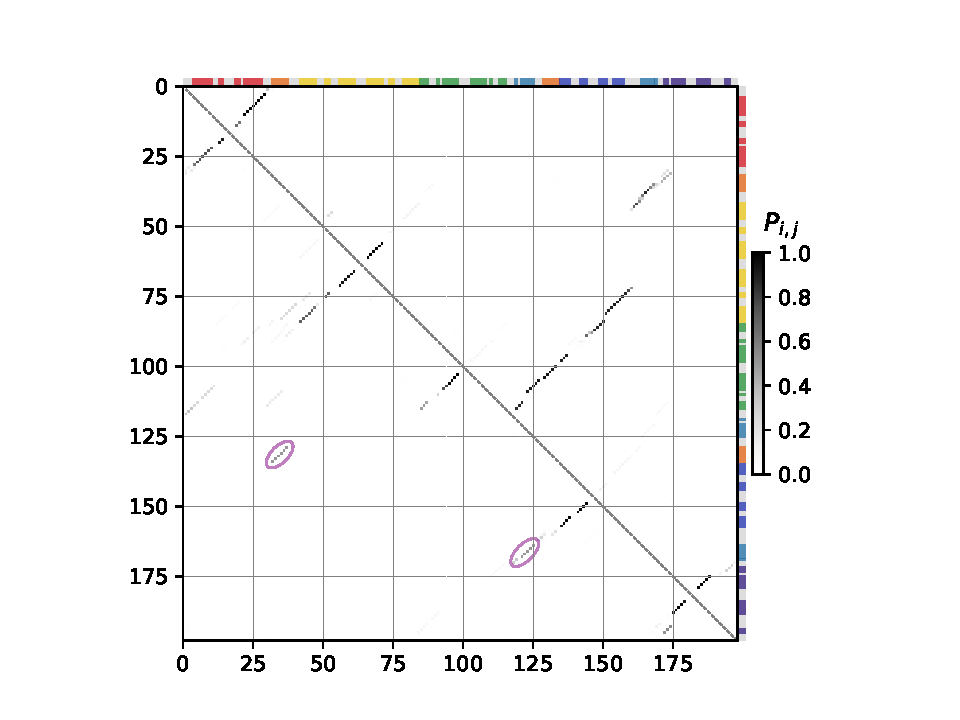
\includegraphics[trim=55 10 70 10, clip, width=\textwidth]{pic/results/designs/dotplots/examples/minimal-range.pdf}
		\caption{\texttt{minimal} constraint set.
		}\label{fig:bpp_pseven:a}
	\end{subfigure}%
	\begin{subfigure}[t]{0.5\textwidth}
		\centering
		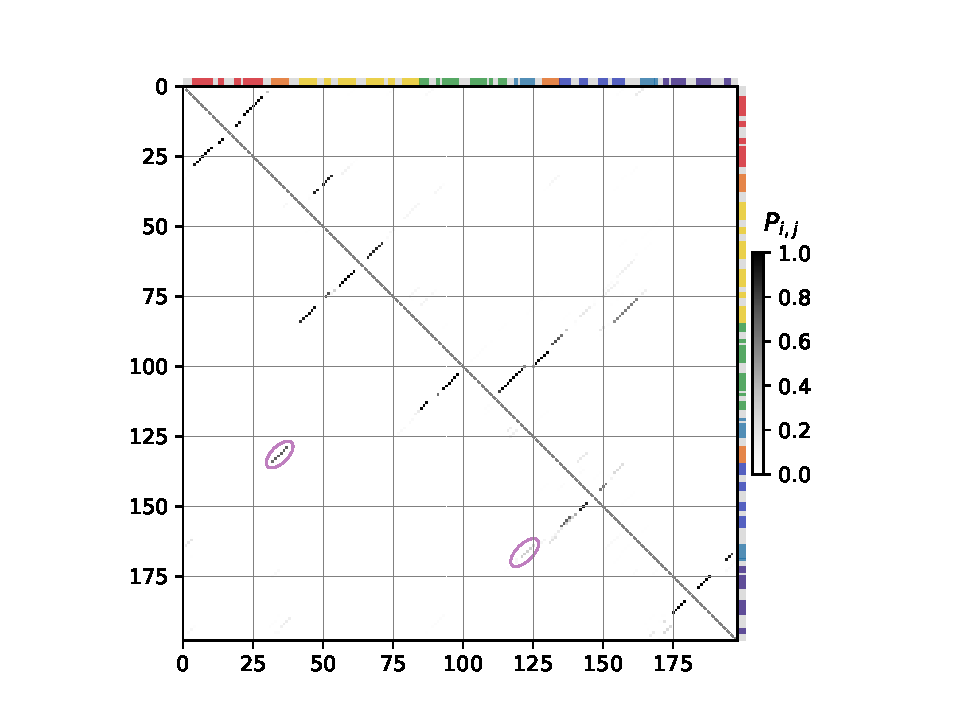
\includegraphics[trim=55 10 70 10, clip, width=\textwidth]{pic/results/designs/dotplots/examples/complete-range.pdf}
		\caption{\texttt{complete} constraint set.
		}\label{fig:bpp_pseven:b}
	\end{subfigure}
	\caption[Base Pair Probabilities of Selected Designs (Constrained Approach)]{
		Base pair probabilities of designed sequences, computed using \texttt{ViennaRNA}. Here, the normalized ensemble defect was used as the objective function.
		\begin{enumerate*}[label={(\alph*)}, font={\bfseries}]
			\item sequence designed with the \texttt{minimal} constraint set
			\item sequence designed with the \texttt{complete} constraint set.
		\end{enumerate*}
		The lower diagonal half of these figures shows one of the best designs in the constraint sets according to the average base pair distance of the three MFE predictions used; the upper diagonal half shows one of the worst designs according to the same metric.
		Position indices of $P_{i,j}$ are labelled at both axes.
		Helices of the native structure are color-coded on top and at the right according to \autoref{fig:azostructure}.
		The location of the original P3-P7 pseudoknot is highlighted in purple.
		See \autoref{tab:examplefasta} for the exact RNA sequences used here.
	}\label{fig:bpp_pseven}
\end{figure}

As visible in the lower diagonal halves of both \autoref{fig:bpp_pseven:a} and \ref{fig:bpp_pseven:b}, sequences considered to be good did in fact show patterns in their base pair probability matrices very similar to the target structure (cf. \autoref{fig:bpp_gissd:a}) including positions of the pseudoknot.
More importantly, these figures illustrate an inherent limitation of this approach; the patterns seen in the upper diagonal halves of \autoref{fig:bpp_pseven:a} and \ref{fig:bpp_pseven:b} do not resemble the target structure in large parts due to the application of structural constraints in the design process.
Specifically, the partition function computation was subject to the same constraints as the MFE structure prediction, effectively leaving P7 positions unpaired (see \autoref{spar:methods:constapproach}).
Conversely, the partition functions computed for Figure \ref{fig:bpp_pseven} were not constrained, effectively allowing nucleotides in P7 to interfere with otherwise carefully optimized positions.
Hence, the constrained approach may produce sequences with structures similar to the target but does not discern unsound designs.

\paragraph{Designs with unconstrained Structure Prediction and alternative Objective Function.}
\label{par:results:unconstrained_maxned}

%\todo{discussion: although the sequence constraint on P7 was removed, we could still include it for the experiments. Removing it illustrates the flexibility of this approach}
%\todo{not sure: merging this with the results for constrained designs seems nicer since I could describe matching figures in parallel BUT: this produces a single rather long subsection if I do not use named paragraphs again. But I don't know fitting names. "Sequence Logos", "Box Plots" and "Dot Plots" is not nice.}

The designs of the sets \texttt{complete-alt} and \texttt{minimal-alt} differ to the previously analyzed sets in the removal of the sequence constraints at P7 and the use of a different objective function (see \autoref{tab:constraintsets}, \autoref{par:methods:ensembledefect}).

Nevertheless, some observations made with the \texttt{complete} and \texttt{minimal} set apply here as well.
The sequence logos of the constraint sets \texttt{complete-alt} and \texttt{minimal-alt} show small conservation at unconstrained positions (Figure \ref{fig:logos_alt}).
Similar to Figure \ref{fig:logos}, both alternative sets of sequence designs show few positions with a single dominating nucleotide identity.
Additionally, there is no evidence in Figure \ref{fig:logos_alt} that the design process favorably produced the nucleotide identities of P7 in the native reference sequence.

\begin{figure}[!ht]
	\centering
	\begin{subfigure}[t]{0.8\textwidth}
		\centering
		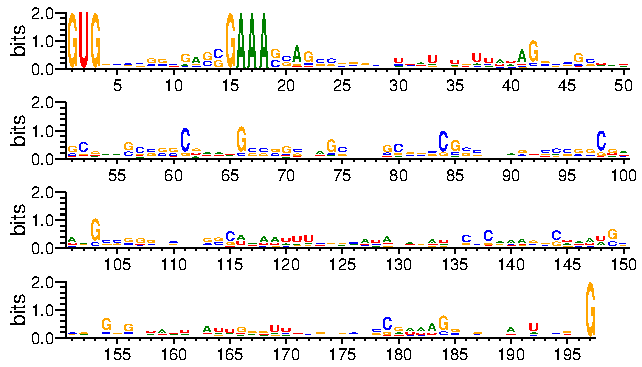
\includegraphics[trim=0 0 0 0, clip, width=\textwidth]{pic/results/designs/logos/logo-minimal-alt.pdf}
		\caption{\texttt{minimal-alt} constraint set.
		}\label{fig:logos_alt:a}
	\end{subfigure}%
	\\
	\begin{subfigure}[t]{0.8\textwidth}
		\centering
		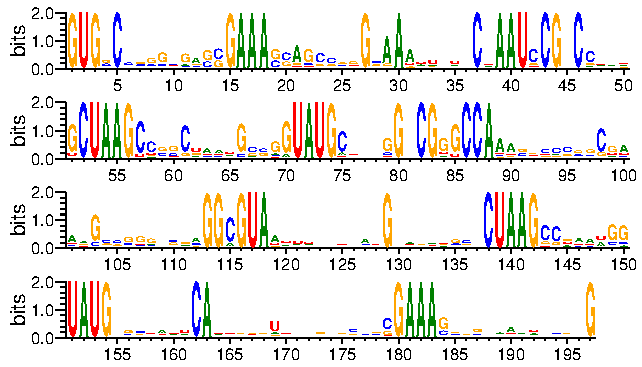
\includegraphics[trim=0 0 0 0, clip, width=\textwidth]{pic/results/designs/logos/logo-complete-alt.pdf}
		\caption{\texttt{complete-alt} constraint set.
		}\label{fig:logos_alt:b}
	\end{subfigure}
	\caption[Nucleotide Composition of Designs (Alternative Approach)]{
		Sequence logos of 
		\begin{enumerate*}[label={(\alph*)}, font={\bfseries}]
			\item sequences designed with the \texttt{minimal-alt} constraint set ($n = 1000$)
			\item sequences designed with the \texttt{complete-alt} constraint set ($n = 1000$).
		\end{enumerate*}
		Nucleotides were colored according to their identity.
		Positions with an information content of \unit[2]{bit} correspond to the sequence constraints.
	}\label{fig:logos_alt}
\end{figure}

\autoref{fig:stats_alt:a} qualitatively resembles \autoref{fig:stats_constrained:a} with differences of the median Hamming distance values attributable to the omission of the P7 sequence constraints.

The minimization of the objective function was stopped at a threshold of $0.15$ as described in \autoref{par:methods:pipelineoverview} (\autoref{fig:stats_alt:b}).
The threshold was chosen higher than in \autoref{fig:stats_constrained:b} to account for the inherent conflict of minimizing the normalized ensemble effect given two superposed target structures. 
%\todo{discussion: this allows a more excellent stop condition than a constant threshold AND: the ED modification allowing pk structures with pk-free partition function would not suffer from this}


\begin{figure}[!ht]
	\centering
	\begin{subfigure}[t]{0.2\textwidth}
		\centering
		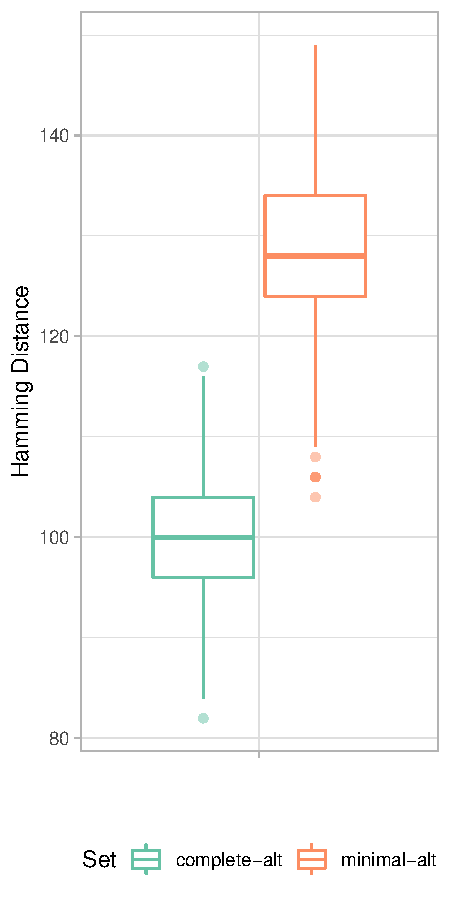
\includegraphics[width=\textwidth]{pic/results/designs/boxplots/alt-hamming-boxplot.pdf}
		\caption{Hamming distance to the native sequence as a measure of sequence similarity.
		}\label{fig:stats_alt:a}
	\end{subfigure}%
	\begin{subfigure}[t]{0.2\textwidth}
		\centering
		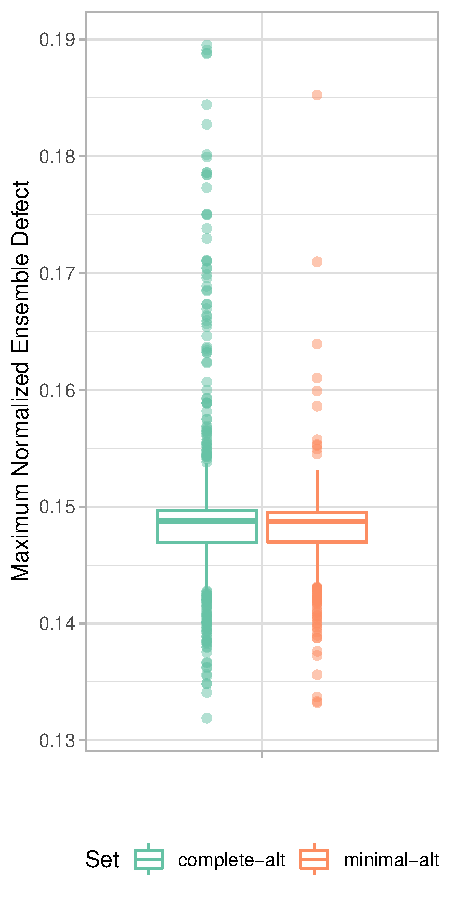
\includegraphics[width=\textwidth]{pic/results/designs/boxplots/alt-score-boxplot.pdf}
		\caption{the maximum normalized ensemble defect of two split target structures (see \autoref{eq:maxned}).
		}\label{fig:stats_alt:b}
	\end{subfigure}%
	\begin{subfigure}[t]{0.27\textwidth}
		\centering
		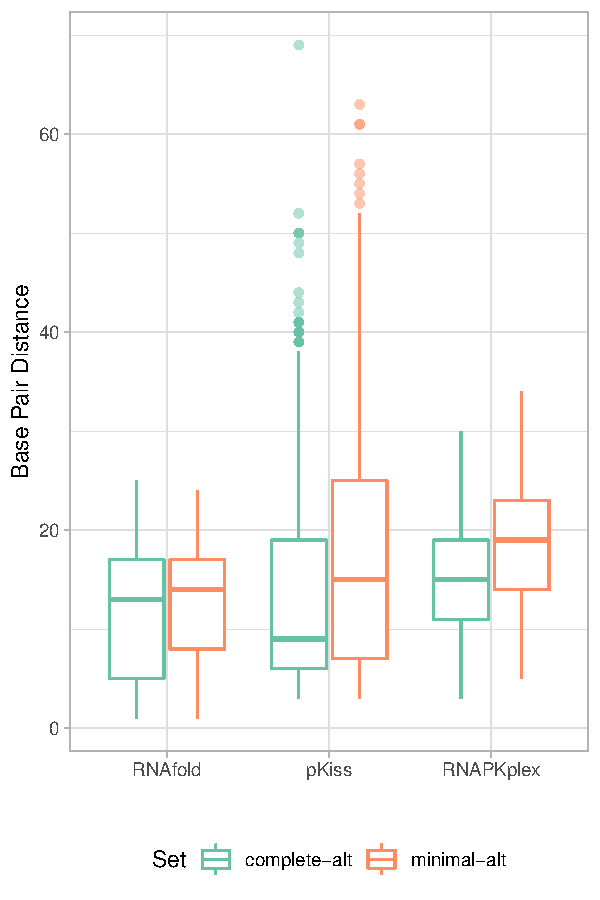
\includegraphics[width=\textwidth]{pic/results/designs/boxplots/alt-bp-boxplot.pdf}
		\caption{Base pair distances relative to the target structure. For predictions made by \texttt{RNAfold}, base pairs of P7 in the target structure were disregarded.
		}\label{fig:stats_alt:c}
	\end{subfigure}
	\begin{subfigure}[t]{0.27\textwidth}
		\centering
		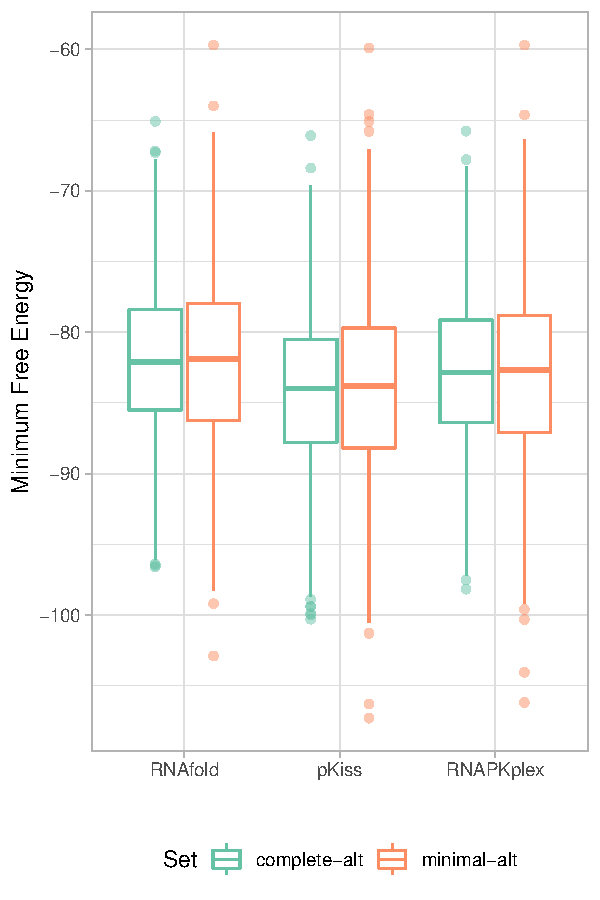
\includegraphics[width=\textwidth]{pic/results/designs/boxplots/alt-mfe-boxplot.pdf}
		\caption{Free Energy of the predicted structures.  \texttt{RNAfold} values were not subject to any correction (cf. \autoref{fig:stats_constrained:d}).
		}\label{fig:stats_alt:d}
	\end{subfigure}
	\caption[Properties of Sequence Designs (Alternative Approach)]{
		Metrics computed for $n = 1000$ sequences designed using the constraint sets \texttt{minimal-alt} and \texttt{complete-alt} respectively.
		No structural constraints were applied for these sequence designs.
	}\label{fig:stats_alt}
\end{figure}

In order to assess the quality of the designed sequences with this approach, the base pair distances relative to the target structure were computed (\autoref{fig:stats_alt:c}).
In contrast to \autoref{fig:stats_constrained:c}, no structural constraints were applied here for the structure prediction with \texttt{RNAfold} since the relevant sequence constraints were omitted as well.
The effect of this choice is immediately visible in \ref{fig:stats_alt:c}, yielding higher values than using the constrained prediction.
However, this was not considered an issue since base pair interactions at positions of the targeted pseudoknot were expected.

Using \texttt{pKiss} and \texttt{RNAPKplex}, structures predicted for sequences using the alternative approach are characterized by a visibly shorter interquartile range than in \autoref{fig:stats_constrained:c}.
Furthermore, the median base pair distance to the target structure is higher for the \texttt{minimal-alt} constraint set, probably due to fewer outliers in comparison with \autoref{fig:stats_constrained:c}.
%This may have been caused by the larger total number of constrained positions in \texttt{complete-alt} reducing complexity or by the fixed nucleotide identities defined by the tertiary interactions, although the latter is very speculative.

Still, the free energies predicted by each of the tools (\autoref{fig:stats_alt:d}) were quite similar to each other and to the results using the constrained approach (see \autoref{fig:stats_constrained:d}).
Contrary to \autoref{fig:stats_constrained:d}, the free energy values for \texttt{RNAfold} were not corrected in any way since not structural constraints were applied.


\begin{figure}[!ht]
	\centering
	\begin{subfigure}[t]{0.5\textwidth}
		\centering
		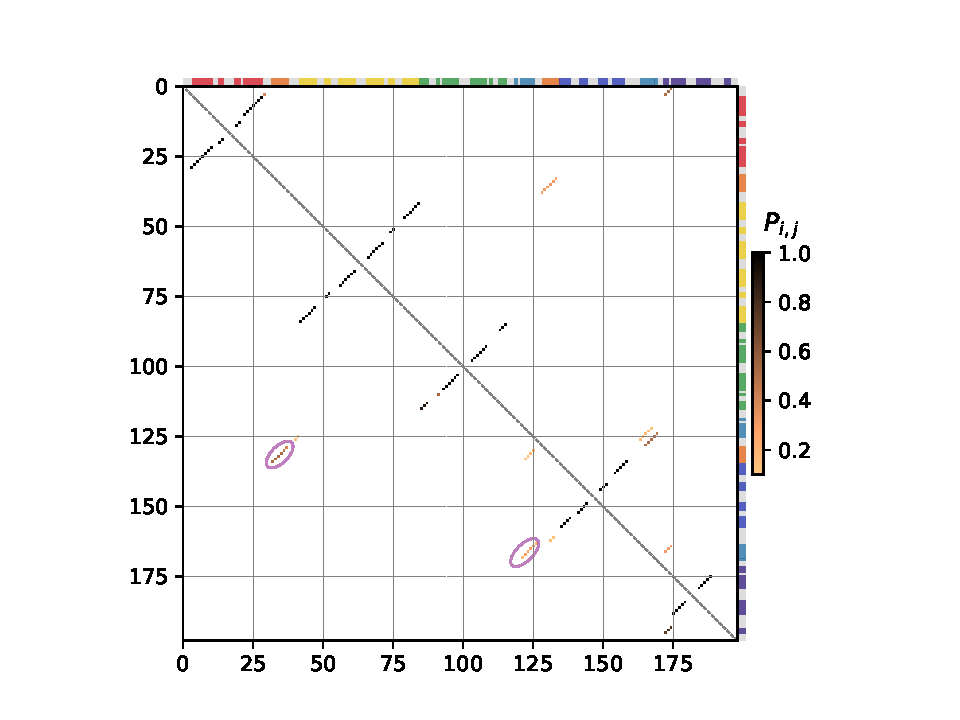
\includegraphics[trim=55 10 70 10, clip, width=\textwidth]{pic/results/designs/dotplots/examples/minimal-alt-rangecolor.pdf}
		\caption{\texttt{minimal-alt} constraint set.
		}\label{fig:bpp_nopseven:a}
	\end{subfigure}%
	\begin{subfigure}[t]{0.5\textwidth}
		\centering
		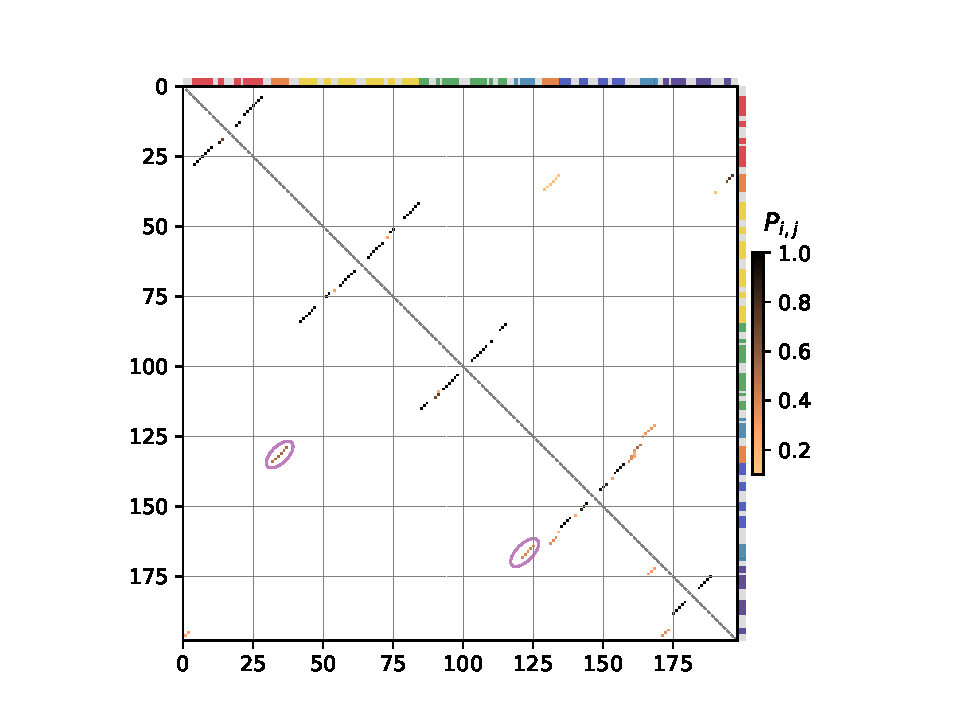
\includegraphics[trim=55 10 70 10, clip, width=\textwidth]{pic/results/designs/dotplots/examples/complete-alt-rangecolor.pdf}
		\caption{\texttt{complete-alt} constraint set.
		}\label{fig:bpp_nopseven:b}
	\end{subfigure}
	\caption[Base Pair Probabilities of Selected Designs (Alternative Approach)]{
		Base pair probabilities of designed sequences, computed using \texttt{ViennaRNA}. For these designs, $\widehat{\operatorname{ned}}_P(s_1^*, s_2^*)$ was used as the objective function (see \autoref{eq:maxned}).
		\begin{enumerate*}[label={(\alph*)}, font={\bfseries}]
			\item sequence designed with the \texttt{minimal-alt} constraint set
			\item sequence designed with the \texttt{complete-alt} constraint set.
		\end{enumerate*}
		The lower diagonal half of these figures shows one of the best designs in the constraint sets according to the average base pair distance of the three MFE predictions used; the upper diagonal half shows one of the worst designs according to the same metric.
		Position indices of $P_{i,j}$ are labelled at both axes.
		Helices of the native structure are color-coded on top and at the right according to \autoref{fig:azostructure}.
		The location of the original P3-P7 pseudoknot is highlighted in purple.
		The location of the original P3-P7 pseudoknot is highlighted in purple. Base pairings with probability $< 0.1$ were omitted and a colored scale was chosen to improve visibility. See \autoref{tab:examplefasta} for the exact RNA sequences used here.
	}\label{fig:bpp_nopseven}
\end{figure}

Just as before, example sequences were selected according to the average base pair distance of the structures predicted using \texttt{RNAfold}, \texttt{pKiss} and \texttt{RNAPKplex}. 
Their base pair probability matrices were computed using \texttt{ViennaRNA} and are shown in Figure \ref{fig:bpp_nopseven}.
A colored scale was chosen, and probabilities below a threshold of $0.1$ were excluded to aid visibility.

Similar to Figure \ref{fig:bpp_pseven}, sequence designs of both \texttt{minimal-alt} and \texttt{complete-alt} considered good closely resemble the target structure including positions of the pseudoknot (see lower diagonal half of Figure \ref{fig:bpp_nopseven}).

The upper diagonal half of both \autoref{fig:bpp_nopseven:a} and \ref{fig:bpp_nopseven:b} still resemble the target structure in large parts and improve drastically upon the previously used constrained approach.
Nevertheless, positions close to the pseudoknot of the target structure seem less well defined in their shape and show lower base pair probabilities than in the lower diagonal half.
In contrast to one of the constrained designs (\autoref{fig:bpp_pseven:a}, lower diagonal half), the \unit[1]{nt} bulge of P7 is not observed here.

%\todo{discussion: implications of those dot plots: pf\_fold and MEA are suited better than MFE prediction for the case of azoarcus GII}


\end{document}
